\subsection{Двовимірні системи та лінійні оператори}

У найзагальнішому вигляді двовимірну систему можна розглядати як математичне відображення (mapping) множини вхідних двовимірних функцій на множину вихідних. Якщо розглядати базовий випадок однозначного відображення (one-to-one mapping), де незалежними неперервними просторовими змінними є $(x, y)$, таку систему можна описати за допомогою загального оператора $O\{\cdot\}$:
\begin{equation}
	G(x, y) = O\{F(x, y)\},
\end{equation}
де $F(x, y)$ --- вхідна функція зображення, а $G(x, y)$ --- результат її перетворення.

Для глибокого аналізу процесів дискретизації та відновлення неперервних функцій (що є основою для побудови цифрових зображень) широко застосовуються сингулярні оператори. Ключовим інструментом тут виступає двовимірна дельта-функція Дірака $\delta(x, y)$, яка має такі фундаментальні властивості:
\begin{equation}
	\int_{-\varepsilon}^{\varepsilon} \int_{-\varepsilon}^{\varepsilon} \delta(x, y) \, dx \, dy = 1 \quad \text{при} \quad \varepsilon > 0,
\end{equation}
\begin{equation}
	\int_{-\infty}^{\infty} \int_{-\infty}^{\infty} F(\xi, \eta) \delta(x - \xi, y - \eta) \, d\xi \, d\eta = F(x, y).
\end{equation}

Останній вираз визначає так звану властивість фільтрації (sifting property) дельта-функції. Вона дозволяє розкласти будь-яку вхідну функцію зображення $F(x, y)$ на нескінченну суму амплітудно-зважених імпульсів Дірака. Сама ж двовимірна дельта-функція є сепарабельною і може бути подана як добуток двох одновимірних функцій за ортонормованими координатами: $\delta(x, y) = \delta(x)\delta(y)$.

Якщо двовимірна система підпорядковується закону адитивної суперпозиції, вона класифікується як лінійна. Для такої системи відгук на суму зважених сигналів дорівнює сумі зважених відгуків на кожен сигнал окремо. Застосовуючи оператор лінійної системи $O\{\cdot\}$ до розкладеної через дельта-функції вхідної функції, порядок застосування оператора та інтегрування можна змінити:
\begin{equation}
	G(x, y) = \int_{-\infty}^{\infty} \int_{-\infty}^{\infty} F(\xi, \eta) O\{\delta(x - \xi, y - \eta)\} \, d\xi \, d\eta.
\end{equation}

Другий множник під інтегралом визначає реакцію системи на ідеальний точковий імпульс і називається імпульсним відгуком (impulse response) двовимірної системи:
\begin{equation}
	H(x, y; \xi, \eta) = O\{\delta(x - \xi, y - \eta)\}.
\end{equation}
В оптичних системах цей параметр також відомий як функція розсіювання точки (point spread function). Підставляючи його у попереднє рівняння, отримуємо інтеграл суперпозиції:
\begin{equation}
	G(x, y) = \int_{-\infty}^{\infty} \int_{-\infty}^{\infty} F(\xi, \eta) H(x, y; \xi, \eta) \, d\xi \, d\eta.
\end{equation}

Адитивна лінійна двовимірна система називається просторово-інваріантною (ізопланатичною), якщо її імпульсний відгук залежить виключно від різниці координат $(x - \xi)$ та $(y - \eta)$. Фізично це означає, що при зміщенні точкового джерела у площині об'єкта, його зображення у фокальній площині також лише зміщується, не змінюючи своєї функціональної форми.

\begin{figure}[h!]
	\centering
	% Вставте сюди вирізану схему з лінзою (Figure 1.2-2 з книги)
	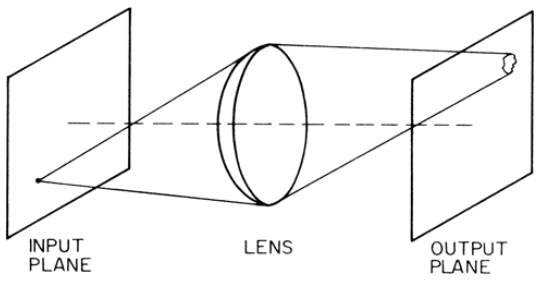
\includegraphics[width=0.7\textwidth]{figures/lens} 
	\caption{Схема формування зображення точкового джерела в оптичній системі}
	\label{fig:point_source}
\end{figure}

Для просторово-інваріантних систем функція імпульсного відгуку спрощується:
\begin{equation}
	H(x, y; \xi, \eta) = H(x - \xi, y - \eta).
\end{equation}
У такому випадку інтеграл суперпозиції зводиться до важливого часткового випадку — двовимірного інтеграла згортки (convolution integral):
\begin{equation}
	G(x, y) = \int_{-\infty}^{\infty} \int_{-\infty}^{\infty} F(\xi, \eta) H(x - \xi, y - \eta) \, d\xi \, d\eta.
\end{equation}
Символічно операція згортки позначається як $G(x, y) = F(x, y) \circledast H(x, y)$.

\begin{figure}[h!]
	\centering
	% Вставте сюди вирізану схему згортки (Figure 1.2-3 з книги)
	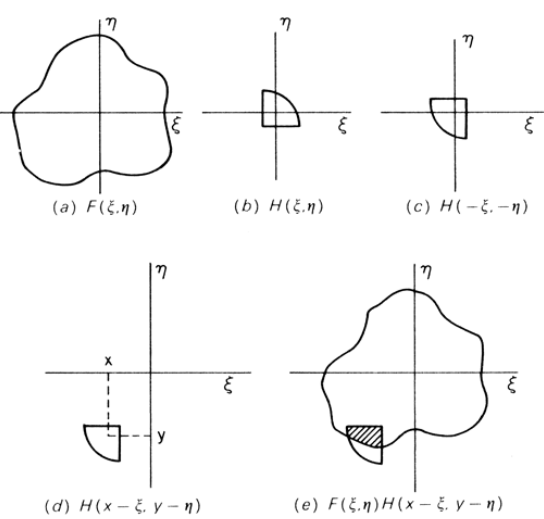
\includegraphics[width=0.8\textwidth]{figures/convolution} 
	\caption{Графічна візуалізація процесу двовимірної згортки}
	\label{fig:convolution_example}
\end{figure}

Процес згортки можна візуалізувати як послідовне сканування вхідної функції $F(x, y)$ інвертованим та зміщеним імпульсним відгуком $H$ з одночасним інтегруванням площі їх перекриття (рис. \ref{fig:convolution_example}). 

У контексті цифрової обробки та масштабування зображень, процес просторової інтерполяції математично споріднений із наведеною теорією. Роль неперервного імпульсного відгуку $H(x, y)$ беруть на себе базисні інтерполяційні функції (наприклад, поліноми Чебишева або барицентричні ядра), які визначають вагу впливу кожного дискретного пікселя (імпульсу) на формування нового, відмасштабованого значення у цільових координатах.